\documentclass{article}

\usepackage{fancyhdr}
\usepackage{extramarks}
\usepackage{amsmath}
\usepackage{amsthm}
\usepackage{amssymb}
\usepackage{amsfonts}
\usepackage{tikz}
\usepackage[plain]{algorithm}
\usepackage{algpseudocode}
\usepackage{graphicx} 
\usepackage{comment}
\usepackage{listings}
\usepackage{courier}
\usepackage[version=3]{mhchem}
\usepackage{wasysym}
\usepackage{subfigure}
\usepackage{enumitem}
\usepackage{physics}
\lstloadlanguages{[5.2]Mathematica}
\lstset{basicstyle=\footnotesize\ttfamily}

\usetikzlibrary{automata,positioning}

%
% Basic Document Settings
%

\topmargin=-0.45in
\evensidemargin=0in
\oddsidemargin=0in
\textwidth=6.5in
\textheight=9.0in
\headsep=0.25in

\linespread{1.1}

\pagestyle{fancy}
\lhead{\hmwkAuthorName}
\chead{\hmwkClass\ (\hmwkClassInstructor,\ \hmwkClassTime): \hmwkTitle}
\rhead{\firstxmark}
\lfoot{\lastxmark}
\cfoot{\thepage}

\renewcommand\headrulewidth{0.4pt}
\renewcommand\footrulewidth{0.4pt}

\setlength\parindent{0pt}

%
% Create Problem Sections
%

\newcommand{\enterProblemHeader}[1]{
    \nobreak\extramarks{}{Problem \arabic{#1} continued on next page\ldots}\nobreak{}
    \nobreak\extramarks{Problem \arabic{#1} (continued)}{Problem \arabic{#1} continued on next page\ldots}\nobreak{}
}

\newcommand{\exitProblemHeader}[1]{
    \nobreak\extramarks{Problem \arabic{#1} (continued)}{Problem \arabic{#1} continued on next page\ldots}\nobreak{}
    \stepcounter{#1}
    \nobreak\extramarks{Problem \arabic{#1}}{}\nobreak{}
}

\setcounter{secnumdepth}{0}
\newcounter{partCounter}
\newcounter{homeworkProblemCounter}
\setcounter{homeworkProblemCounter}{1}
\nobreak\extramarks{Problem \arabic{homeworkProblemCounter}}{}\nobreak{}

%
% Homework Problem Environment
%
% This environment takes an optional argument. When given, it will adjust the
% problem counter. This is useful fo when the problems given for your
% assignment aren't sequential. See the last 3 problems of this template for an
% example.
%
\newenvironment{homeworkProblem}[1][-1]{
    \ifnum#1>0
        \setcounter{homeworkProblemCounter}{#1}
    \fi
    \section{Problem \arabic{homeworkProblemCounter}}
    \setcounter{partCounter}{1}
    \enterProblemHeader{homeworkProblemCounter}
}{
    \exitProblemHeader{homeworkProblemCounter}
}

%
% Homework Details
%   - Title
%   - Due date
%   - Class
%   - Section/Time
%   - Instructor
%   - Author
%

\newcommand{\hmwkTitle}{Homework\ \#5}
\newcommand{\hmwkDueDate}{Friday, Nov. 5, 2016 at 6:00pm}
\newcommand{\hmwkClass}{CS 187}
\newcommand{\hmwkClassTime}{Section 1}
\newcommand{\hmwkClassInstructor}{Prof. Perona}
\newcommand{\hmwkAuthorName}{Albert Ge }

%
% Title Page
%

\title{
    \vspace{2in}
    \textmd{\textbf{\hmwkClass:\ \hmwkTitle}}\\
    \normalsize\vspace{0.1in}\small{Due\ on\ \hmwkDueDate\ at 2:00pm}\\
    \vspace{0.1in}\large{\textit{\hmwkClassInstructor,\ \hmwkClassTime}}
    \vspace{3in}
}

\author{\textbf{\hmwkAuthorName} }
\date{}

\renewcommand{\part}[1]{\textbf{\large Part \Alph{partCounter}}\stepcounter{partCounter}\\}


%
% Various Helper Commands
%

% Useful for algorithms
\newcommand{\alg}[1]{\textsc{\bfseries \footnotesize #1}}

% For derivatives
\newcommand{\deriv}[1]{\frac{\mathrm{d}}{\mathrm{d}x} (#1)}

% For partial derivatives
\newcommand{\pderiv}[2]{\frac{\partial}{\partial #1} (#2)}

% Integral dx
\newcommand{\dx}{\mathrm{d}x}

% Alias for the Solution section header
\newcommand{\solution}{\textbf{\large Solution}}

% Probability commands: Expectation, Variance, Covariance, Bias
\newcommand{\E}{\mathrm{E}}
\newcommand{\Var}{\mathrm{Var}}
\newcommand{\Cov}{\mathrm{Cov}}
\newcommand{\Bias}{\mathrm{Bias}}

\begin{document}

\maketitle

\pagebreak

\begin{homeworkProblem}
    \section{1. }
    \subsection{a. }
    On a high level, a speech recognition model takes the audio waveform of speech and breaks it down to a vector of values. For a feedforward network, these values be fed into a network structure with weight factors that determine how important a particular input element is. Since there are no loops in a feedforward network structure, the input elements can be propagated through the network without having to revisit units in the network; this leads to a fairly straightforward computation, using techniques of gradient descent and backpropagation to update the weights accordingly, to better accomodate the data. \\
    For recurrent neural networks, the primary difference is that the structure is not limited by loops in the network. Instead of computing the values layer by layer (as in a feedforward case), the network is computed by time steps. At each time step, values are computed according to the weights and architecture of the network, and the state of the network is saved. In this way, information learned in past time steps can be recalled and used in future computations, which can assist in making better predictions about the data. \\
    The advantage afforded by recurrent networks over feedforward architecture is primarily to use past knowledge to make decisions about what the audio input was trying to say. Intuitively, it can be helpful to understand the context of a sentence before trying to identify a word from the sound produced, or to interpret what the word means relative to the rest of the sentence. RNNs directly provide this ability, because past time steps, which can correspond to past audio inputs, can be retrieved to help classify the new input.\\

    \subsection{b. }
    An important feature of recurrent neural networks is being able to produce an arbitrary number of outputs. In the case of object-classification in images, it may be unclear how many objects can be classified. Recurrent neural networks can potentially classify more objects by virtue of the potentially unlimited number of time steps. At each time step, an output is produced, corresponding to probabilities of object-classifications. Thus, the advantage afforded over feedforward networks is that the recurrent neural network can continually produce output, whereas the feedforward network is rigid and can only produce as many classifications as are predefined. \\
    One advantage that feedforward neural networks have, however, is that their structure allows them to easily stack layers and layers upon another. An important layer that is used in image processing is the convolution layer, which produces feature maps that describe general patterns in 2-dimensional data. In other words, the convolutional neural network takes advantage of the 2-dimensionality of the input, to make better predictions about what the image represents.\\
    To blend these models, we may think of creating a convolutional recurrent neural network. The input image could be first fed through convolutional layers to produce the feature maps, and then fed into a recurrent neural network. This would allow the network to better visualize patterns in the data, while also being able to classify an arbitrary number of objects that a recurrent neural network affords.


\section{2. }
The partial derivative of loss w.r.t. a hidden state at some time $t$ can be written as
\[
    \pdv{\mathcal{L}}{h_t} = \pdv{h_{t+1}}{h_t}\pdv{h_{t=2}}{h_{t+1}}\cdots \pdv{o_T}{h_T}\pdv{L}{o_T}
\]
Intuitively, the state of $h_t$ is being updated through backpropagation of the error on the output at the final time $T$.
Given the recursive formula of $h_t$, we can rewrite
\[
    \pdv{\mathcal{L}}{h_t} = W_{hh} \tanh'(W_{hh} h_t + W_{xh}x_t + b_h) \cdot W_{hh} \tanh'(W_{hh} h_{t+1} + W_{xh}x_{t+1} + b_h) \cdots W_{hh} \tanh'(W_{hh} h_{T-1} + W_{xh}x_{T-1} + b_h) + W_{hy}
\]
For each time step $t$, a derivative tanh function is applied. The tanh function graphed looks like this:
\begin{figure}[H]
    \centering
    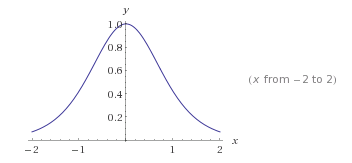
\includegraphics[]{tanh}
\end{figure}
Notice that, for nonzero values of tanh, the output is less than 1. Since it is probabilistically unlikely to have zero uniformly when multiplying the weight matrix with the input and the previous hidden state, many of these tanh terms will come out to be less than 1. Thus, for very early hidden states with $t << T$, the gradient computed through backpropagation is extremely diluted from the partial of the loss function on time $T$. As a result, the gradients 'vanish', meaning that the first few hidden states get updated much more slowly, and the network trains very slowly. \\
Long short-term memories can help prevent this by storing protected 'memory', so that it can be recalled, without contamination, at any time step. The basic structure of a LSTM unit consists of a keep gate, write gate, and read gate; these gates perform operations on the stored memory; either to keep it, overwrite it, or retrieve it. Thus, during the backpropagation step, the error derivative can be saved inside the memory cell, and kept over many steps, without worrying about the tanh derivative terms diluting it. 




\section{3. }
\begin{lstlisting}
Temperature:  0.25
they each seized a broomstick and kicked off into  he the the the  he the t th th the the g th the g the s the  he the the the the  he the  on the ge t t s t the the the the the th the the th the  he t the g th t the t th t the n the the the the g th
Temperature:  0.75
they each seized a broomstick and kicked off into h  he he tt  ie h ho gil d th t  an , sol on th t t ton  the e the g cwe t d. th wa ch ml thm he the s, thou ,  id rn. the  son the  th nos be s we thy he -t re the s t the wn t  hoo bt no d  oy pt re
Temperature:  1.5
they each seized a broomstick and kicked off into thkun t,d.ngi ,emwow?at uith the god' ri wha reame go", o bt.a,t yg-

al" fdmllbl.twi ". gr tet
"e pner 
had wl
 fsmlen, ano
,?".
te, aa,, vepre hnd
!

\end{lstlisting}



\begin{lstlisting}
----- temperature: 0.25
Temperature:  0.25
they each seized a broomstick and kicked off into the stand of the dark as they was a be all out a secoune the stope the starter on the firet of the care shat it had and sair and de all the stope serment. he was a still on the wall bedine hermione wa
Temperature:  0.75
they each seized a broomstick and kicked off into the camors.

"i've gotten on i was a fange of the shay. harry strect there wording to have hermione sated them that the
sheet shopped and he nerve been read were authing she hished he'd lome the stall
Temperature:  1.5
they each seized a broomstick and kicked off into frender their faugled and know it's weep from likeh
late from msabos with an his meped this
budfbry.
wharper mug,h mameds. her yeg.opli's faffrised fffffatcale ftulleys hakeny. plem you pebcrats thoug
\end{lstlisting}
Qualitatively, the generated sequences appear to use longer, more complete words during training. For example, for a temperature of 0.25, the first epoch mostly uses words with the letter 't', and most often the word 'the'. By the 20th epoch, many more complete words are apparent, such as 'all', 'and', 'hermione'. At higher temperatures the predictions are more incoherent, as the words formed are not valid English words, and the use of punctuation characters are more apparent. 
    

\end{homeworkProblem}

\begin{homeworkProblem}
\section{1. }
Generative adversarial networks basically use two networks: a network that only generates data from an existing dataset, and a second network that discriminates whether the data received is from the original dataset, or from the generated network. Based on the predictions of the discrimatory network, the generative network can take that and adjust its parameters so that future data produced would become less and less predictable for the discriminatory network, until it does no better than random guessing between the true and generated data. \\
Auto-regressive models, in general, produce output based on previous values. The parameters are the weights assigned to each of the previous values. In the example of a PixelRNN, the network is given an incomplete image; these incomplete pixels serve as the 'previous values', and are trained on to generate the next of layer of pixels. This can be recursively applied to complete the entire image. \\
Finally, latent variable models are used to relate the data to latent variables, which are not observable, and are inferred from other observed variables. For example, in generating image of digits, latent variable models first decide a target digit (the latent variable) before generating the image for that digit. The exact parameters for generating the digit are unknown (thus 'latent'), and the model is trained by increasing the likelihood of approximating these latent variables given the data. In the case of variational auto-encoders (VAE), the model is trained by maximizing the likelihood that the latent variable distribution given generated data approximate the latent variable distribution given the actual data.\\
The model used in problem 1.3 most closely aligns with the auto-regressive model. This is because each character in the seed sequence can be thought of as a 'previous value', that contributes some weight into predicting the next character in the sequence. 

\section{2. }
We begin with the marginal log-likelihood, $\log p(x) = \sum_z q(z | x) \log(p(x))$, since $\sum_z q(z|x) = 1$. The joint probability distribution tell us that
$p(x, y) = p(y|x)p(x)$, for continuous random variables, so we have that
\[
\sum_z q(z | x) \log(p(x))  = \sum_z q(z | x) \log(\frac{p(x, z)}{p(z|x)}) =
\sum_z q(z | x)\log(\frac{p(x, z)}{q(z|x)}\frac{q(z|x)}{p(z|x)})
\]
\[
=\sum_z q(z | x)\log(\frac{p(x, z)}{q(z|x)}) + \sum_zq(z|x) \log\frac{q(z|x)}{p(z|x)}
\]
% Notice that the second term is just expected value, conditioned on the distribution $q(z|x)$. We have
% \[
% \mathbb{E}_{q(z|x)}\log\frac{q(z|x)}{p(z|x)} \geq \log( \mathbb{E}_{q(z|x)}[\frac{q(z|x)}{p(z|x)}])
% \]
% by Jensen's inequality, as log is a convex function.
The second term is defined to be the KL divergence from $q(z|x)$ to $p(z|x)$. The KL divergence has a property of being nonnegative (Gibb's inequality), so giving us the bound
$\log p(x) \geq \sum_z \log(\frac{p(x, z)}{q(z|x)})$.
Using Bayes' theorem, this term can be written as
\[
\sum_z q(z|x)\log(\frac{p(x, z)}{q(z|x)}) = \sum_z q(z|x)\log(\frac{p(x|z)p(z)}{q(z|x)}) = 
\sum_zq(z|x)\log(\frac{p(z)}{q(z|x)}) + \sum_zq(z|x)\log(p(x|z))
\]
The first term, by definition, is just the negative KL divergence from $q(z|x)$ to $p(z)$. The second term is just expected value, conditioned on the distribution $q(z|x)$. Thus we have
$\log p(x) \geq -D_{KL}(q(z|x)||p(z)) + \mathbb{E}_{q(z|x)}[\log p(x|z)]$.

The KL-divergence can be thought of as a regularization term; it is being subtracted from the lower-bound, so it can be thought of a penalty term for how well the model is fitting the data (i.e. the minimum guarantee of the marginal log-likelihood of the data). The second term is the expected reconstruction error; it measures the log-probability of replicating $x$ from $z$. If $z$ can perfectly reproduce $x$, then then the expected error is zero.

\section{3. }
The variational lower bound for both the training and testing sets were plotted as a function of the number of epochs.
\begin{figure}[H]
    \centering
    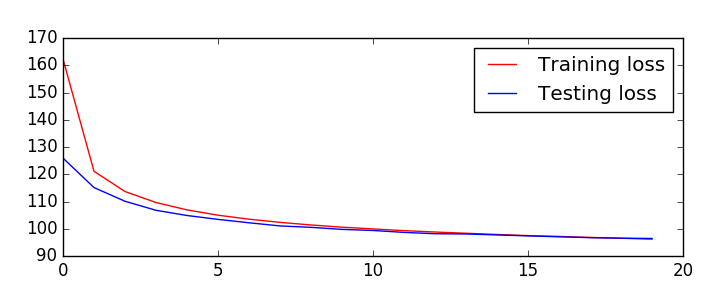
\includegraphics[width=15cm]{error.png}
\end{figure}
The figure shows that losses from both training and testing at first drop quickly, then slowly level out. \\
For the reconstruction images, ten samples of different digits were collected and redrawn using the trained VAE network. As the number of epochs increases, the pictures drawn become more clearer and sharper, which is indicative of the model's confidence of the digit drawn. 
\begin{figure}[H]
    \centering
    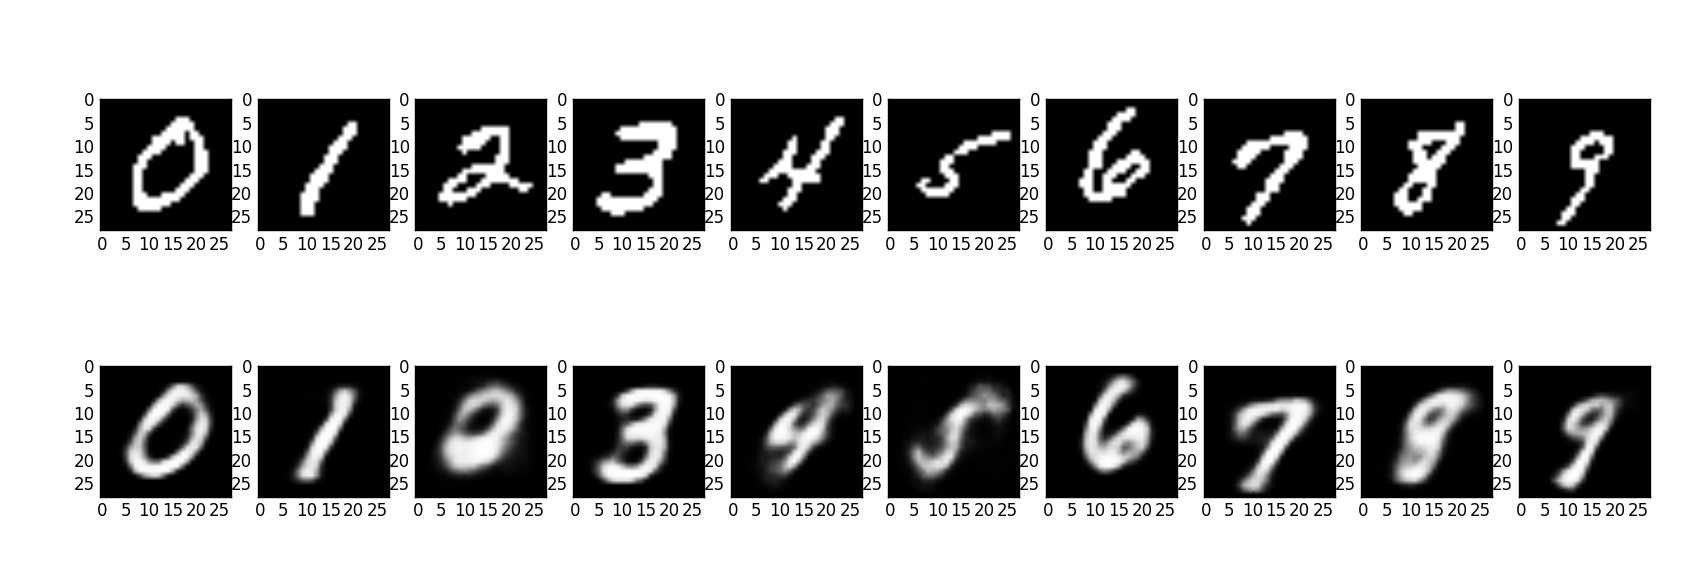
\includegraphics[width=13cm]{1.png}
    \caption{Training with one epoch}
\end{figure}


\begin{figure}[H]
    \centering
    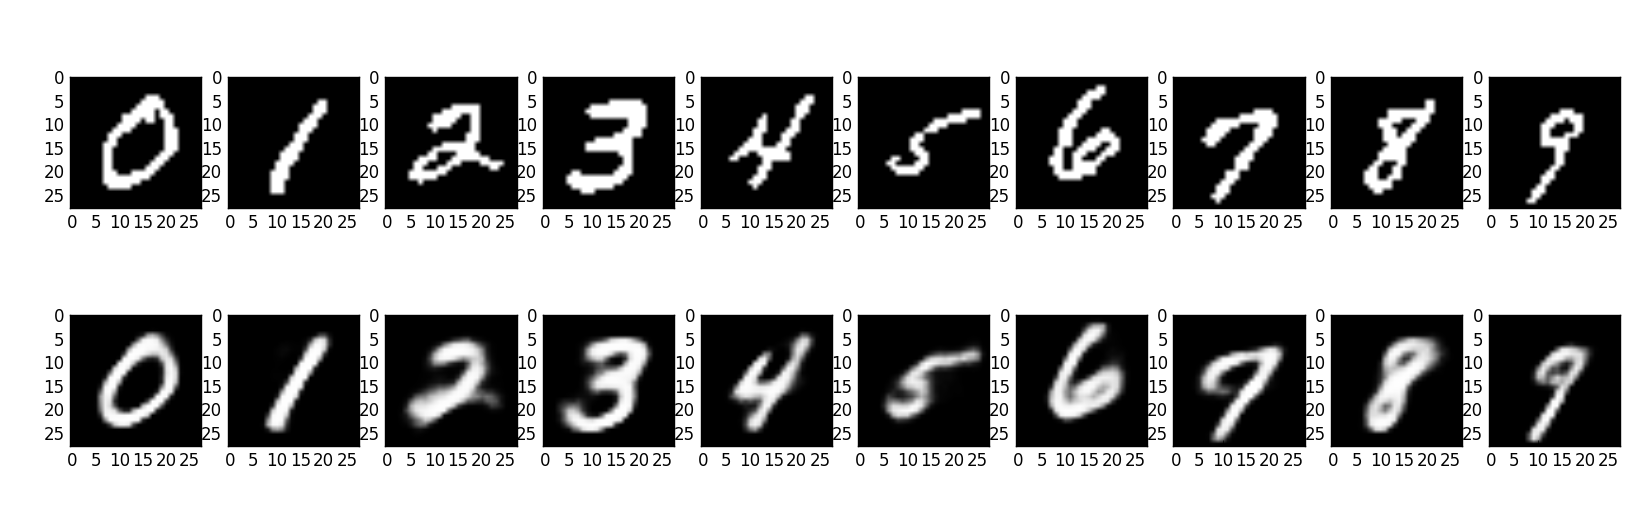
\includegraphics[width=13cm]{2.png}
    \caption{Training with ten epochs}
\end{figure}

\begin{figure}[H]
    \centering
    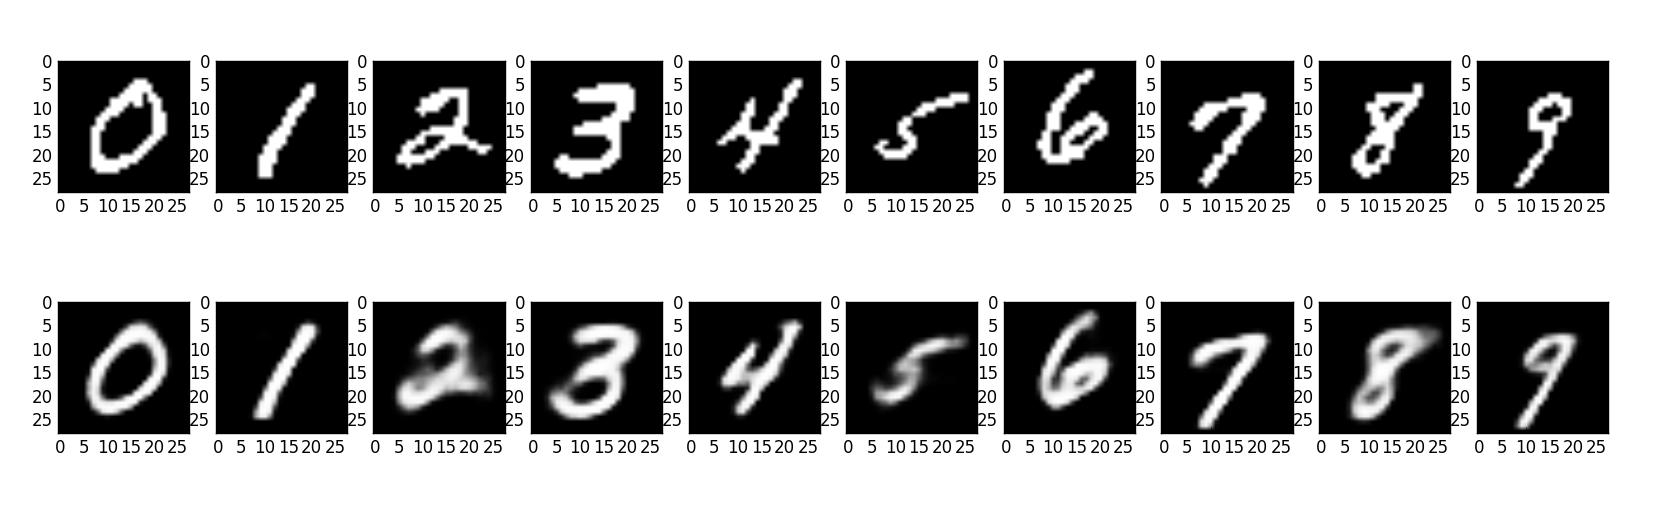
\includegraphics[width=13cm]{3.png}
    \caption{Training with twenty epochs}
\end{figure}


\end{homeworkProblem}

\end{document}
